\documentclass{beamer}
\usepackage{graphicx}
\usepackage[T1]{fontenc}
\usepackage[polish]{babel}
\usepackage{csquotes}
\usepackage[style=authortitle,backend=biber]{biblatex}
\usepackage{hyperref}
% chktex-file

\graphicspath{ {./images/} }
\usetheme{Warsaw}
\addbibresource{references.bib} 
\setbeamertemplate{navigation symbols}{}

\title[Twierdzenie o reprezentancie]{Twierdzenie o reprezentancie \textendash{} zastosowanie w analizie danych}
\author{Jakub Dyrcz}
\institute{Studenckie Koło Naukowe Matematyków Politechniki Krakowskiej}
\date{\today}
\logo{
\includegraphics[height=1cm]{logo}}

\newtheorem{definicja}{Definicja}
\newcommand{\imagesize}{0.7\textwidth}
\newcommand{\imagestandard}[1]{\includegraphics[width=\imagesize]{#1}}
\newcommand{\norm}[1]{\left\lVert#1\right\rVert}
\newcommand{\Hilbert}{\ensuremath{\mathcal{H}}}
\newcommand{\zeroinfty}{\ensuremath{\left[0, +\infty\right)}}
\newcommand{\bb}[1]{\ensuremath{\mathbb{#1}}}


\begin{document}
\maketitle

\section{Wprowadzenie}
\begin{frame}{Wstęp}
  \only<1>{
    Weźmy zbiór danych $I = \{(x_1, y_1), \ldots, (x_n, y_n) : (x_i,  y_i) \in  \bb{R}^2\}$, gdzie para ($x_i$, $y_i$) to obserwacja.

    \begin{figure}
      \centering
      \imagestandard{wykres1.png}
    \end{figure}
  }
  \only<2>{
    Dobrym pomysłem byłoby znalezienie jakiejś krzywej, która aproksymowałaby wszystkie wartości $y_i$ w punkcie $x_i$. Niech $f$ będzie \textbf{funkcją aproksymującą}:
  \begin{equation}
    y_i = f(x_i) + \varepsilon_i,
  \end{equation}
  gdzie $\varepsilon_i$ to szum, który jest różnicą między pomiarem $y_i$ a stanem faktycznym. Typowym przykładem zaszumionych danych mogą być np. dane z\ pomiaru\ temperatury, gdzie termometr może mieć własny błąd pomiarowy. W związku z tym zakładamy, że 
  \[\mathbb{E}[\varepsilon_i] = 0.\]
  }
\end{frame}
\section{Regresja}
\begin{frame}{Regresja}
  \only<1>{
     Widać wyraźnie, że poniższe dane układają się w prostą, dlatego najlepszym pomysłem będzie użycie funkcji liniowej $f$:
    \[
      f(x) = \alpha + \beta{x}.
    \]
    Funkcję tej postaci nazywamy \textbf{prostą regresji}.
    \begin{figure}
      \centering
      \imagestandard{wykres1.png}
    \end{figure}
  }
  \only<2>{
    Dobierając odpowiednie parametry $\alpha$ i $\beta$ możemy uzyskać prostą, która będzie najlepiej przybliżać obserwacje - czynność ta nazywa się \textbf{regresją}.
      
        \begin{figure}
          \centering
          \imagestandard{wykres2.png}
        \end{figure}
  }
  \only<3>{
    Do wyznaczenia tej prostej użyto metody najmniejszych kwadratów. Szukamy takich parametrów $\alpha_i$ i $\beta_i$, dla których zachodzi:
    \[\min_{\alpha,\beta \in \bb{R}}{ \sum_{i=1}^{n} {(y_i - f(x_i))}^{2}}.\]
    \begin{figure}[h]
      \centering
      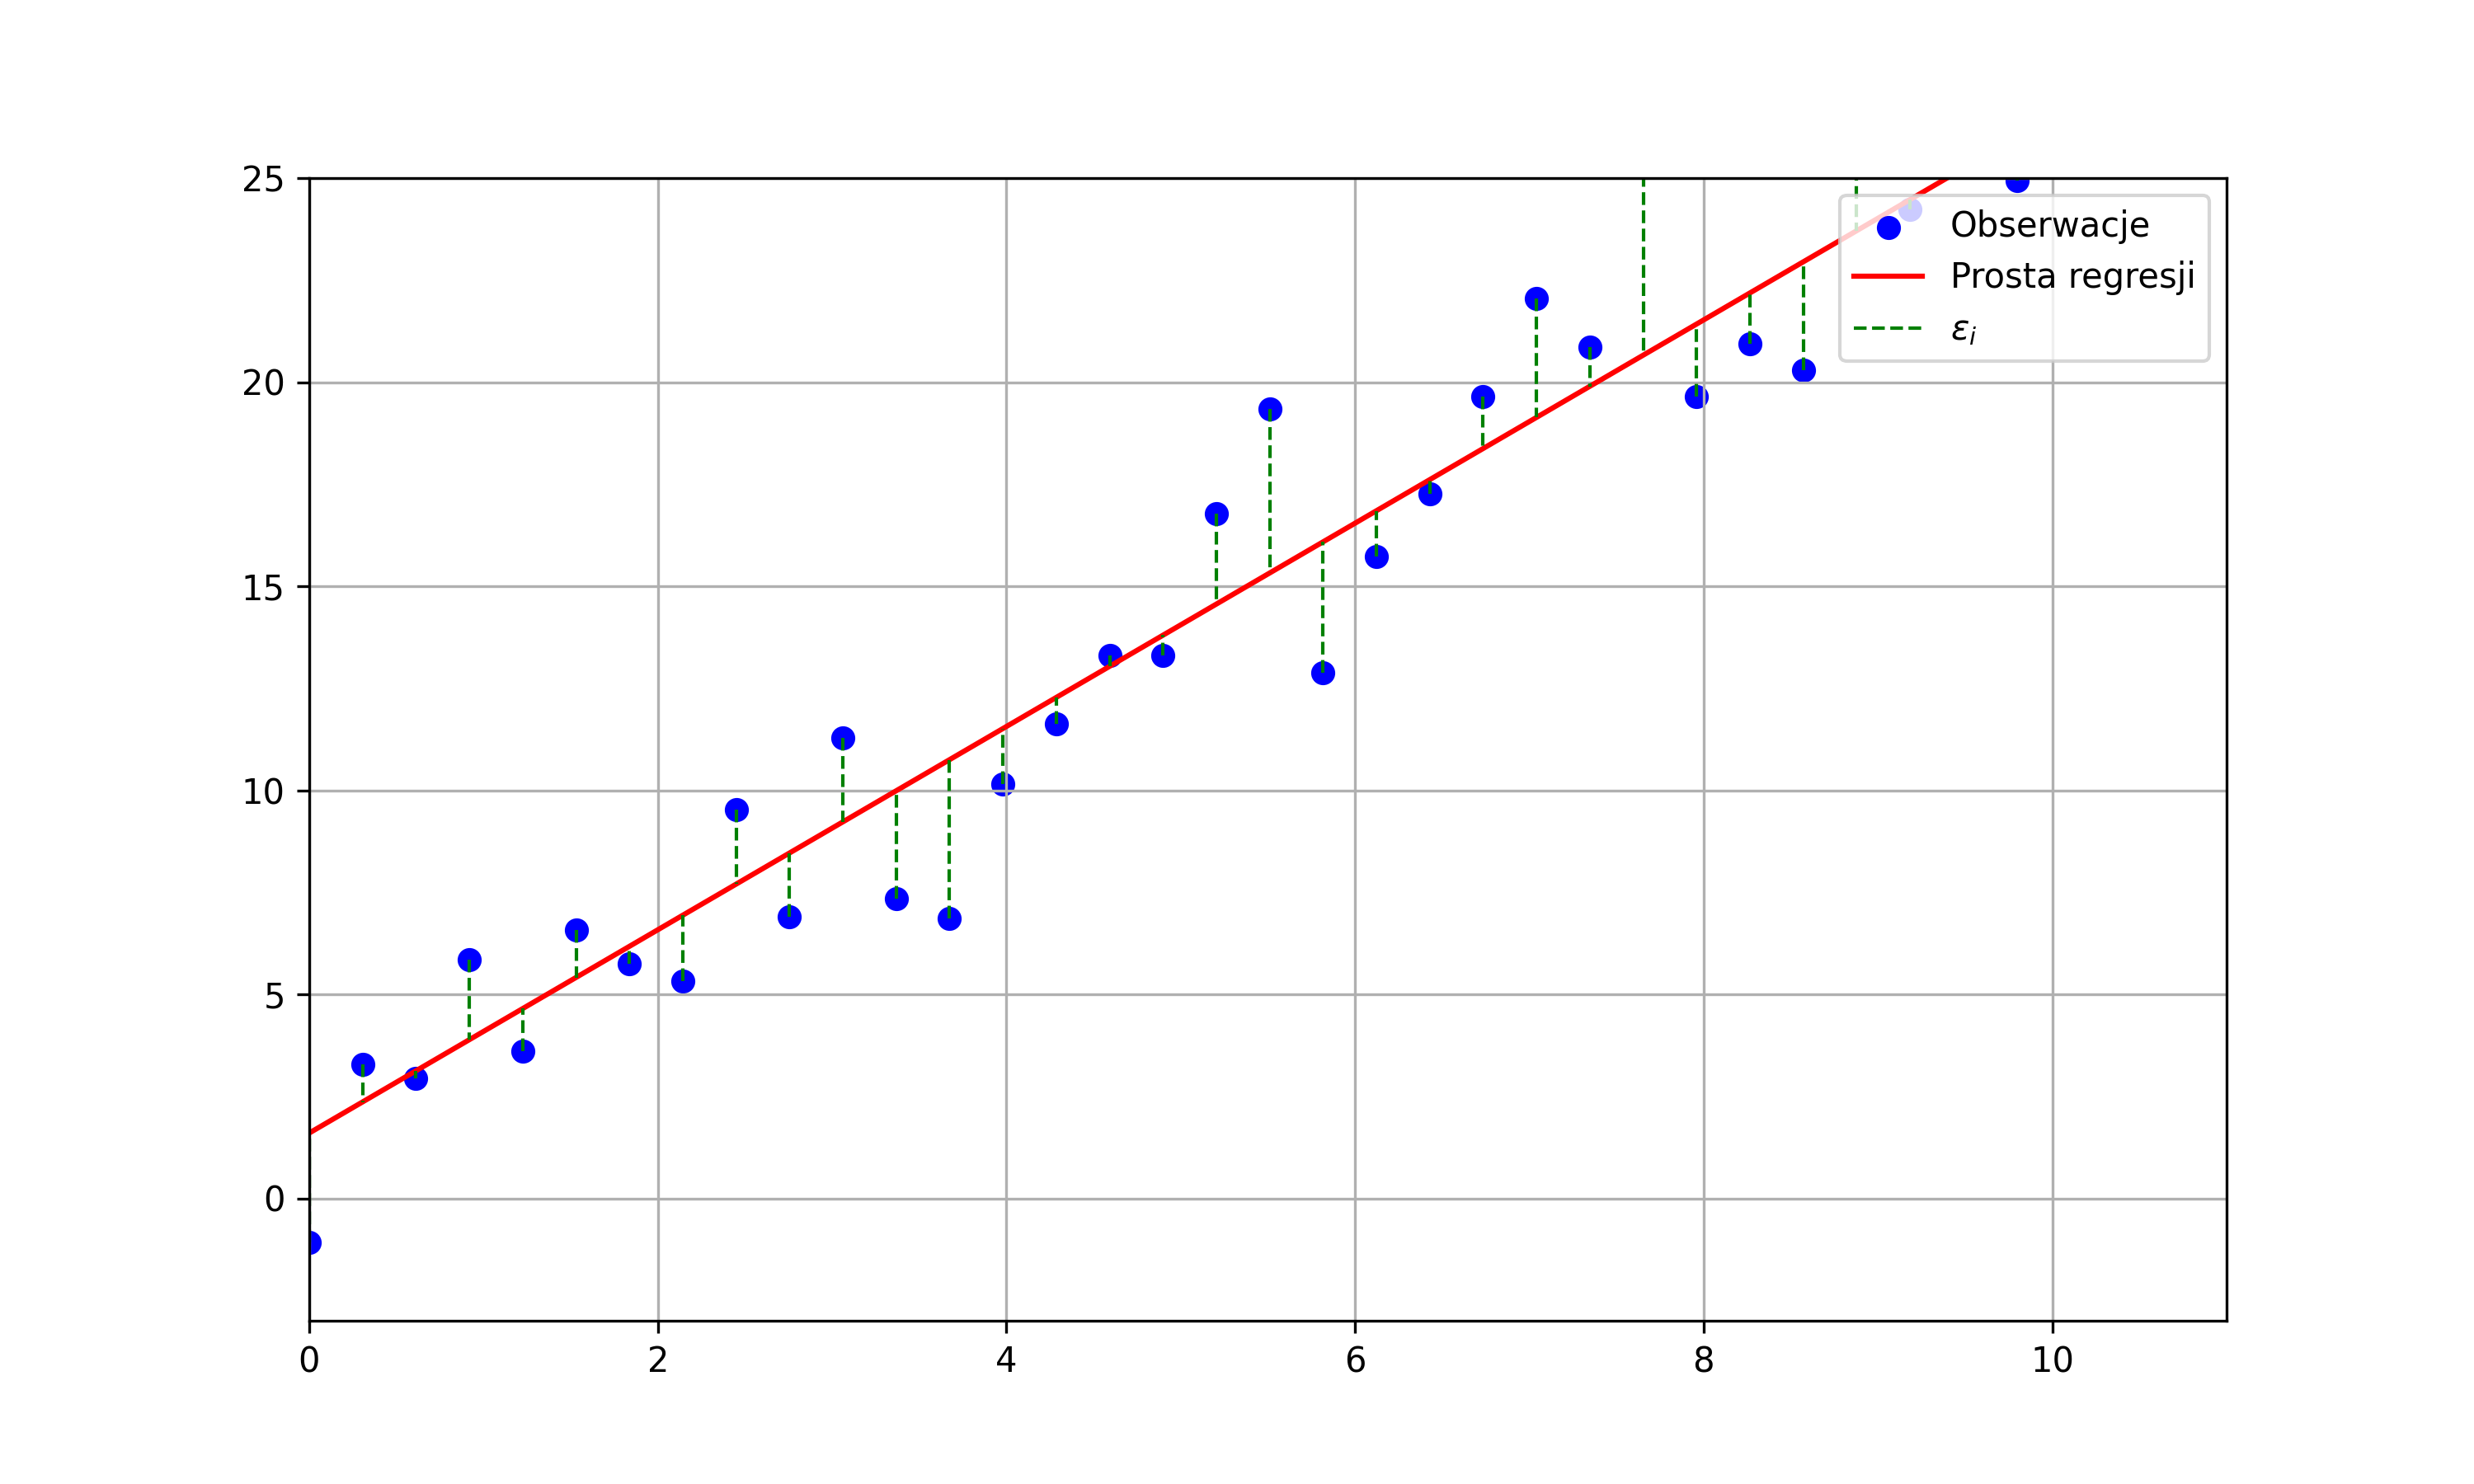
\includegraphics[width=0.6\textwidth]{wykres3.png}
    \end{figure}
  }
\end{frame}

\begin{frame}{Regresja bardziej złożonych danych}
  \only<1>{A co w przypadku, kiedy dane przyjmują kształt bardziej złożonej krzywej? Szukanie wtedy ręcznie funkcji jest bezcelowe. Lepszym pomysłem jest użycie interpolacji i skorzystanie z danych które mamy, aby potraktować je jako węzły.}
  \only<2>{Warto zwrócić uwagę, że nie każda interpolacja będzie dobra. W przypadku, gdy użyjemy interpolacji kawałkami liniowej, to w pewnych punktach pojawią się wierzchołki, w których funkcja nie będzie różniczkowalna. Dużo lepszym pomysłem byłoby użycie interpolacji Lagrange'a.}
  \only<3>{Jednakże mając $n$ węzłów otrzymamy wielomian stopnia $n - 1$. W związku z tym, że węzłów możemy mieć naprawdę wiele, to taki wielomian szybko stanie się bezużyteczny.
  }
  \begin{figure}
    \centering\label{fig:wykres}
    \only<1>{\imagestandard{wykres4.png}} 
    \only<2>{\imagestandard{wykres8.png}}
    \only<3>{\imagestandard{wykres5.png}}
  \end{figure}
\end{frame}

\begin{frame}{Regresja \textendash{} jaka powinna być?}
  Zanim pójdziemy dalej, przeanalizujmy cechy, które powinna mieć dobra krzywa regresji:
  \begin{itemize}
    \item<1-> gładka,
    \item<2-> łagodna,
    \item<3-> funkcja powinna dobrze aproksymować dane.
  \end{itemize}
\end{frame}
\begin{frame}
  \begin{figure}
    \centering
    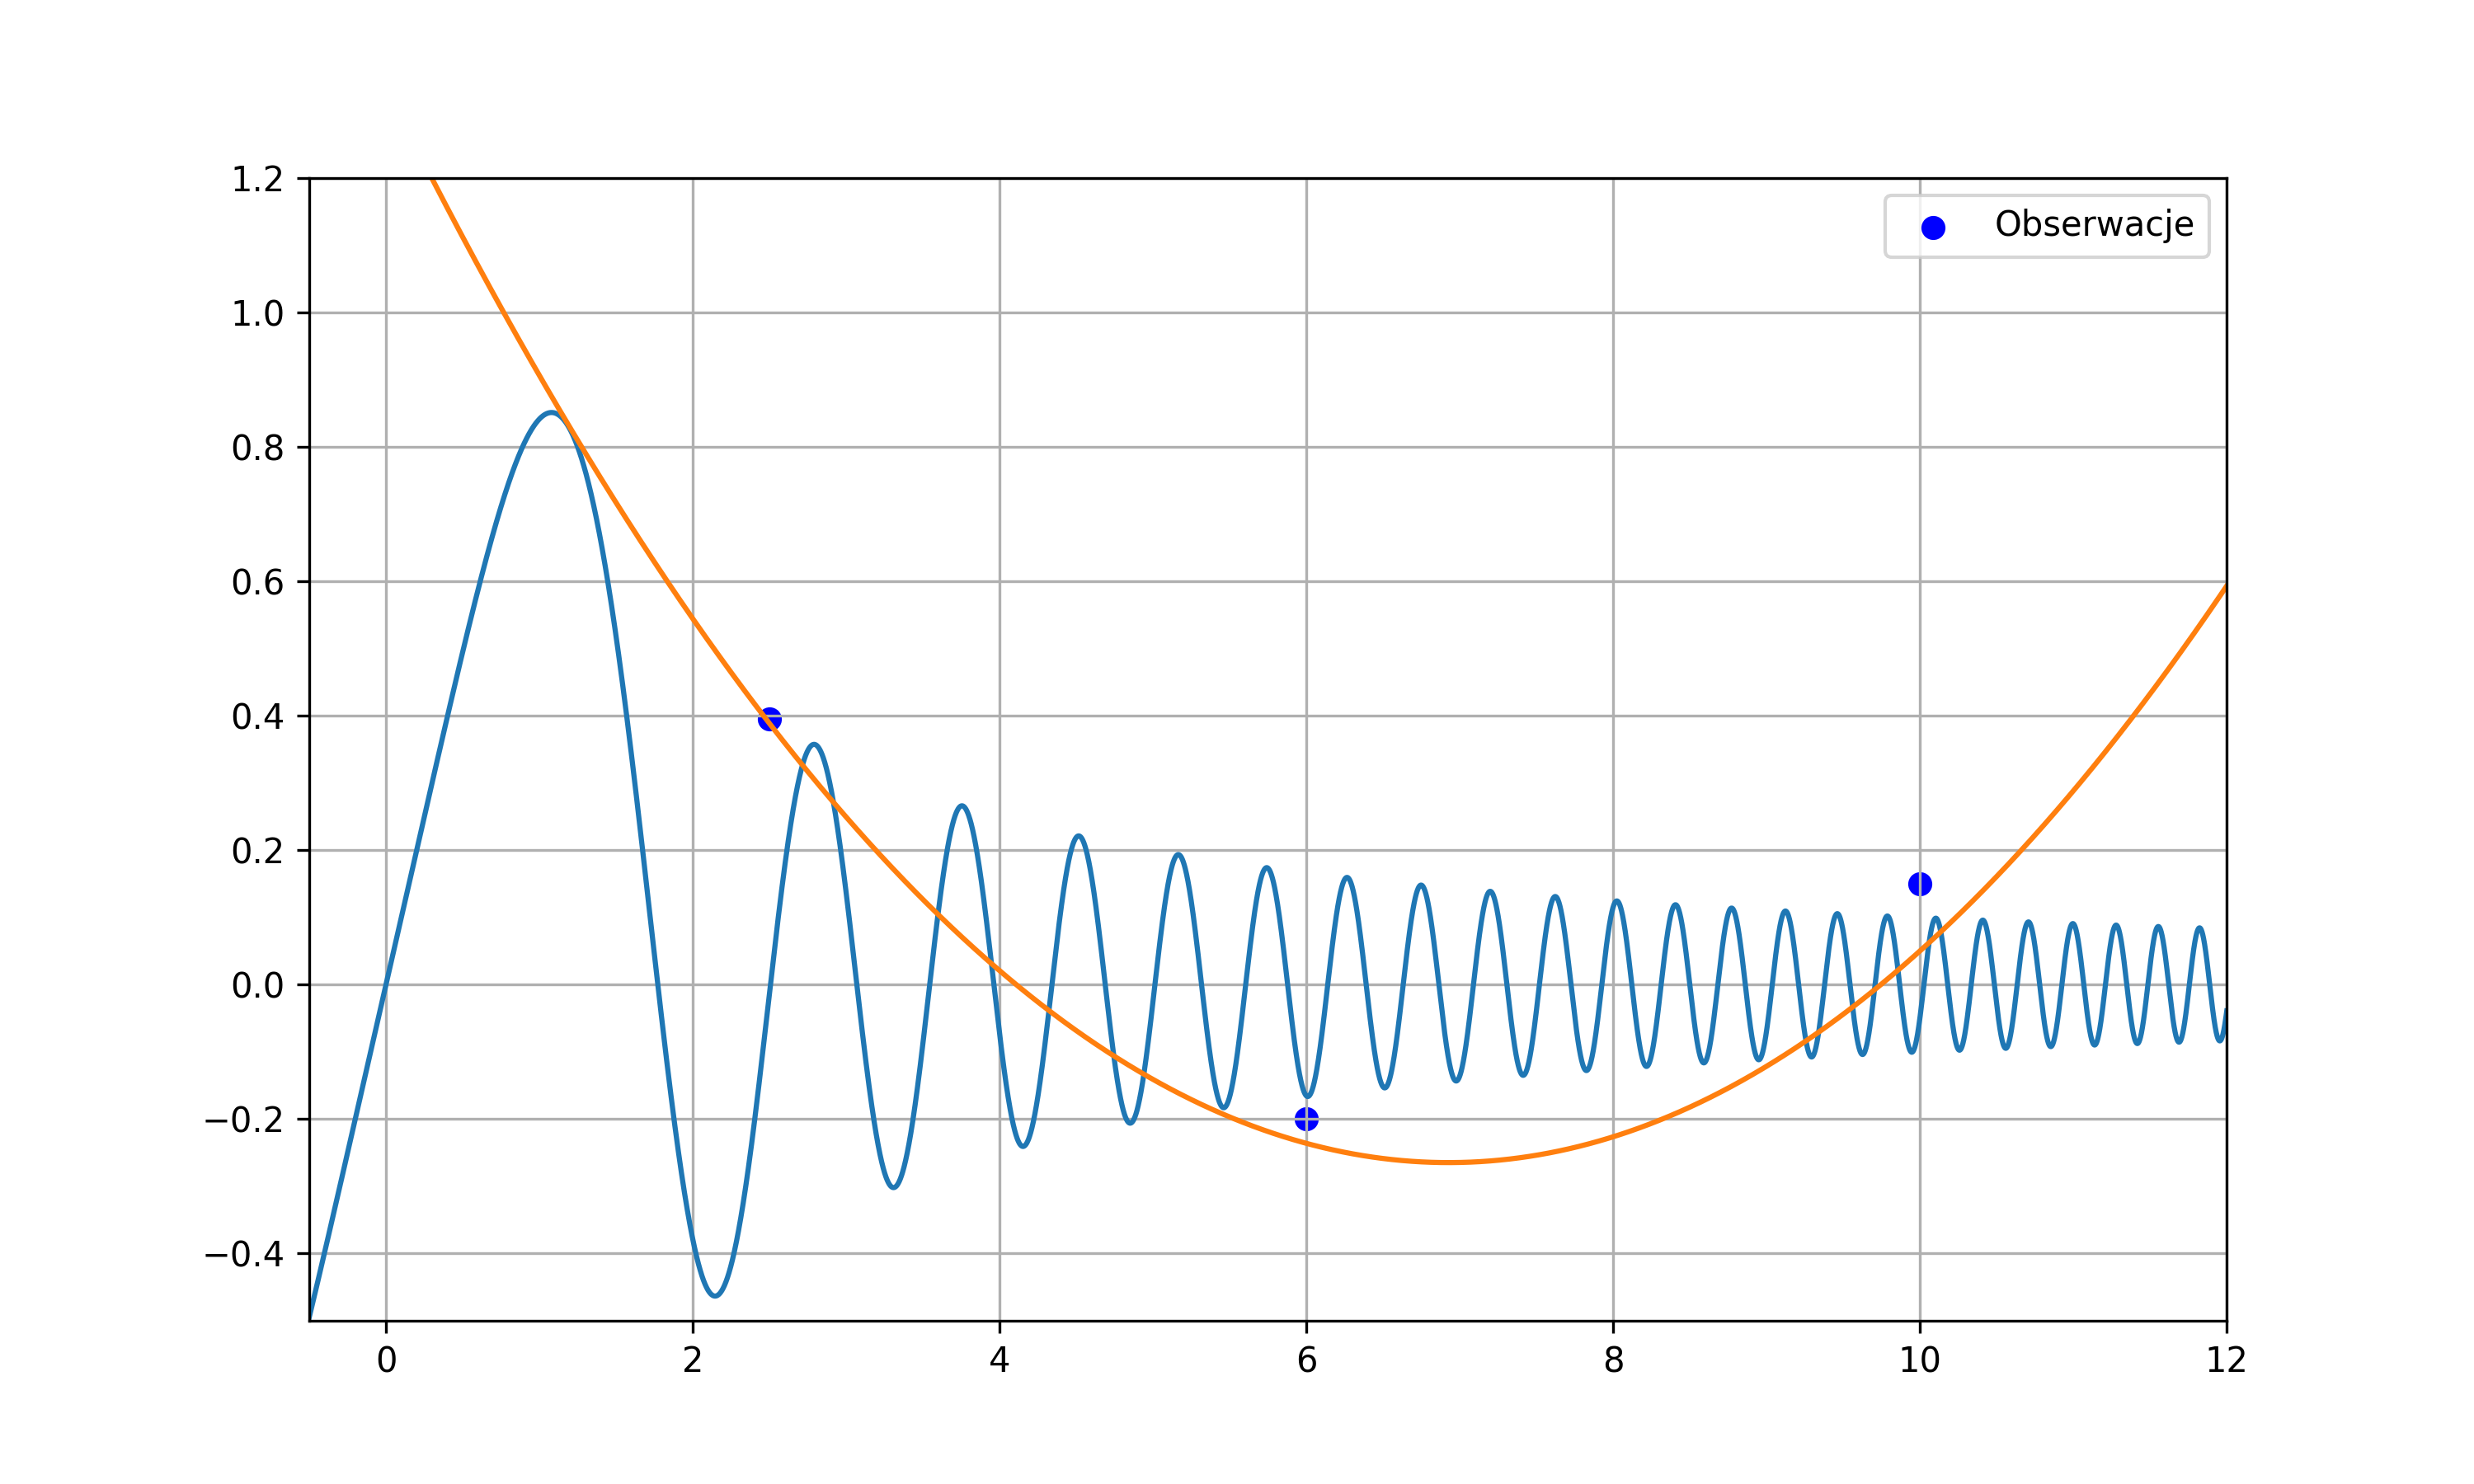
\includegraphics[width=1\textwidth]{wykres9.png}
  \end{figure}
\end{frame}

\section{Przestrzeń Hilberta}
\begin{frame}[allowframebreaks]{Definicje}
\begin{definicja}
  \textbf{Przestrzeń Hilberta} to przestrzeń wektorowa $\mathcal{V}$ (nad ciałem $\bb{R}$ lub $\bb{C}$), która:
  \begin{itemize}
    \item ma zdefiniowany iloczyn skalarny $\langle \cdot, \cdot \rangle$,
    \item przestrzeń $\mathcal{V}$ z metryką indukowaną przez $\langle \cdot, \cdot \rangle$, jest zupełna.
  \end{itemize}
\end{definicja}
\begin{definicja}
  \textbf{Przestrzeń Hilberta z jądrem reprodukującym (RKHS)} to przestrzeń Hilberta $\Hilbert$, której elementami są funkcje $f: \mathcal{X} \rightarrow \bb{K}$, wyposażona w jądro reprodukujące $K: \mathcal{X} \times \mathcal{X} \rightarrow \bb{K}$ takie, że
  \[
    \forall_{x \in \mathcal{X}} \forall_{f \in \Hilbert} \langle f, K(\cdot, x) \rangle = f(x).
  \]
\end{definicja}
\end{frame}


\begin{frame}
\begin{block}{Własność}
  Niech $\Hilbert_1, \Hilbert_2$ będą przestrzeniami Hilberta, ich sumą prostą  $\Hilbert_1 \bigoplus \Hilbert_2 \equiv \Hilbert$ nazywa się przestrzeń Hilberta, która:
  \begin{itemize}
    \item jest sumą prostą przestrzeni wektorowych $\Hilbert_1$ i $\Hilbert_2$,
    \item ma zdefiniowany iloczyn skalarny \\ 
    \vspace{2mm}
    $\langle (x_1, x_2),(y_1, y_2) \rangle_{\Hilbert} = \langle x_1, y_1 \rangle_{\Hilbert_1} + \langle x_2, y_2 \rangle_{\Hilbert_2}$, \\ 
    \vspace{2mm}
    $x_1, y_1 \in \Hilbert_1, x_2, y_2 \in \Hilbert_2$. \\ 
    \end{itemize}
\end{block}
\end{frame}
 

\section{Twierdzenie o reprezentancie}
\begin{frame}{Regresja metodą najmniejszych kwadratów}
\only<1>{Niech $\mathcal{H}$ będzie RKHS nad ciałem $\mathbb{R}$, składającą się z funkcji określonych na zbiorze $\mathcal{X}$. Niech ponadto $K$ będzie jądrem reprodukującym dla $\mathcal{H}$. Weźmy zbiór obserwacji $\{(x_1, y_1),  \ldots, (x_n, y_n) : x_i \in \mathcal{X}, y_i \in \mathbb{R}\}$. Naszym celem jest możliwie dobre zaaproksymowanie tych obserwacji za pomocą funkcji $f \in \mathcal{H}$:

$$y_i = f (x_i) + \varepsilon_i,\quad \mathbb{E} (\varepsilon_i) = 0.$$
}

\only<2>
{
Ponieważ $\Hilbert$ zazwyczaj jest przestrzenią nieskończenie wymiarową, potrzebujemy pewnego oszacowania. Oszacujemy funkcję $f$ za pomocą metody najmniejszych kwadratów z karą (PLS).

  \begin{equation} \label{eq:PLS}
    \min_{f \in \Hilbert} \left\{ \dfrac{1}{n}\sum_{i=1}^{n}{(y_i - f(x_i))}^2 +  P(f) \right\}
  \end{equation}
  Pierwsza część bada dopasowanie do danych. Odpowiednio dobrana funkcja $P: \Hilbert  \rightarrow \zeroinfty$ karze $f$ za bycie niezbyt łagodną.
}
\end{frame}

\begin{frame}{Twierdzenie o reprezentancie}
  \only<1>{Niech teraz $\Hilbert = \Hilbert_0 \bigoplus \Hilbert_1$, gdzie $\Hilbert_0 = \{ f : P(f) = 0\}$. Przypuśćmy, że $\Hilbert_0$ jest przestrzenią skończenie wymiarową o bazie $\phi_1, \ldots, \phi_m$. Niech ponadto $\tilde{K}$ będzie jądrem repr. dla $\Hilbert_1$.
  }
  \only<-2>{
  
  \begin{alertblock}{Twierdzenie o reprezentancie \textit{(Representer theorem)}}
    Rozwiązaniem problemu~(\ref{eq:PLS}), $\hat{f}$, jest kombinacja liniowa funkcji $\phi_1, \ldots, \phi_m$ i $\tilde{K}(\cdot, x_1), \ldots, \tilde{K}(\cdot, x_n)$:
    \[
      \hat{f}(x) = \sum_{i=1}^{m} {\alpha_i \phi_i(x)} + \sum_{j=1}^{n} {\beta_j \tilde{K}(\cdot, x_j)}.
    \]  
  \end{alertblock} 
  }
  \only<2->
  {
    \begin{block}{Wniosek}
    Jeśli $\Hilbert_0 = \{0\}$ to:
    \[
      \hat{f}(x) = \sum_{j=1}^{n} {\beta_j \tilde{K}(\cdot, x_j)}.
    \]
  \end{block}
  }
\end{frame}
\begin{frame}{Metoda wyznaczania stałych}
  Na potrzebny dalszych obliczeń założmy, że $P(f) = \lambda\norm{f}^2, \lambda \in \bb{R}_+$. Wówczas $\Hilbert_0 = \{0\}$. Teraz pozostaje tylko znaleźć stałe $\beta_j$. Korzystając z regresji grzbietowej otrzymujemy równanie:
  \begin{equation} \label{eq:matrix}
    \begin{pmatrix} y_1 \\ y_2 \\ \vdots \\ y_n \end{pmatrix} = 
    \left(\left(\begin{matrix}
      K(x_1, x_1)  & \cdots & K(x_1, x_n) \\
      K(x_2, x_1)  & \cdots & K(x_2, x_n) \\
      \vdots       &  \ddots & \vdots \\
      K(x_n, x_1)  & \cdots & K(x_n, x_n)
    \end{matrix}\right)
    + \lambda \mathbb{I}_n
    \right) \begin{pmatrix} \beta_1 \\ \beta_2 \\  \vdots \\ \beta_n \end{pmatrix}.
  \end{equation}
\end{frame}
\begin{frame}[allowframebreaks]{W poszukiwaniu jąder reprodukujących}
  Jednym z najpopularniejszych jąder reprodukujących jest jądro Gaussa:
  \[
    K(x, y) = \exp{\left(-\dfrac{\norm{x - y}^2}{2\sigma^2}\right)}.
  \]
  Wyróżniamy jednak też inne jądra reprodukujące, takie jak:
  \begin{itemize}
    \item jądro wielomianowe w RKHS $\mathcal{P}_d(\bb{R})$ wielomianów stopnia co najwyżej $d$:
    \[
      K(x, y) = (\langle x, y\rangle + c)^d, \quad c \geq 0, d \in \bb{N},
    \]
    \item jądro Laplace'a: 
    \[
      K(x, y) = \exp{\left(-\dfrac{\norm{x - y}}{\sigma}\right)}, \quad \text{wraz z}
    \] 
    \[
      \norm{f}^2 = \int_{\bb{R}}\frac{1}{\sigma}{f(x)^2 + \sigma f'(x)^2dx}.
    \]
  \end{itemize}
  My jednak zostaniemy przy jądrze Gaussa, które jest najczęściej używane w praktyce.
\end{frame}

\begin{frame}{Przykład zastosowania twierdzenie o reprezentancie}
  Korzystając teraz z równania~(\ref{eq:matrix}) możemy wyznaczyć $\beta_j$. Poniżej zaprezentowane są wyniki aproksymacji punktów $x_1, x_2, x_3$, dla wartości $\lambda = 0.1$ i $\lambda = 0.5$ (pastelowy~kolor).
  \begin{figure}
    \centering
    \only<1>{\imagestandard{wykres6.png}}
  \end{figure}
\end{frame}

\begin{frame}
Wracając do problemu aproksymacji danych (\ref{fig:wykres}). Kiedy użyjemy twierdzenia o reprezentancie, uzyskamy idealną krzywą regresji. Poniżej przedstawione są wyniki dla $\lambda = 0.1$ i $\lambda = 0.5$ (pastelowy kolor).
\begin{figure}
  \centering
  \only<1>{\imagestandard{wykres7.png}}
\end{figure}

\end{frame}
\section{Podsumowanie}
\begin{frame}{Zastosowanie}
  Twierdzenie o reprezentancie mimo że może się wydawać mało przydatne, to znalazło zastosowanie w wielu dziedzinach, takich jak:
  \begin{itemize}
    \item<1-> uczenie maszynowe,
    \item<2-> statystyka,
    \item<3-> rozwiązywanie równań różniczkowych \textendash{} metoda spektralna,
    \item<4-> interpolacji,
    \item<5-> rekonstrukcji obrazu.
  \end{itemize}
\end{frame}

\begin{frame}{ }
  Dziękuję za uwagę!
\end{frame}

\begin{frame}[allowframebreaks]{Bibliografia}
    \nocite{*}
    \printbibliography{}
\end{frame} 
\end{document}